%%%%%%%%%%%%%%%%%%%%%%%%%%%%%%%%%%%%%%%%%%%%%%%%%%%%%%%%
%%%%                                              %%%%%%
%%%%  Author: Peter Wilson                        %%%%%%
%%%%                                              %%%%%%
%%%%  Stability analysis
%%%%                                              %%%%%%
%%%%%%%%%%%%%%%%%%%%%%%%%%%%%%%%%%%%%%%%%%%%%%%%%%%%%%%%


%fref generates automatically the respective abreviation/word in the text for the reference. You just have to define a label starting with the respective keyword.
%english: chap, sec, fig, eq, app
%deutsch: chap/kap, abs, abb, gl, anh
%see http://ctan.space-pro.be/tex-archive/macros/latex/contrib/fancyref/fancyref.pdf for more \section

%\onehalfspacing
%\setlength{\belowcaptionskip}{-17pt}

\chapter{Stability analysis}
\label{chap:chapter_2_2}

\renewcommand{\Thema}{Stability analysis}

\lettrine[lines=2]{T}{he} expedient practical design of engineering structures is often considered fulfilled after the proper confirmation of allowable deflections and stresses throughout the entire domain. Although the design may in fact be adequate in the vast majority of cases, structural stability is an oft overlooked phenomena in "bread and butter" engineering analysis and is by no means guaranteed by acceptable displacements and stresses. Indeed, some of the most catastrophic structural failures such as the Tacoma Narrows Bridge (1940) and the Twin Towers (2001) have root  causes stemming from system instability and reinforce the importance of stability analysis.

Structural stability, expressed crudely, can be thought of as "the power to recover equilibrium", or, alternatively, a structure can be thought stable at an equilibrium position if it returns to that position following a temporary perturbation \cite{FelippaStabilityBasics2016}. In terms more relatable, it's clear a person standing on one foot is more susceptible to falling over in the presence of a strong wind than someone firmly planted with both feet. Although the person with both feet planted may sway and bob, they have a greater chance to return to their original equilibrium position after the wind has subsided, that is, they are more stable. In an engineering context, perhaps the most well known stability problem is a long beam subject to a compressive end load. At low load levels the beam will undergo small deformations and trace back to it's original configuration after unloading, however, after the critical Euler buckling load is surpassed structural stability is lost giving way to large arbitrary deformations with non-coincident loading and unloading paths. Although these two simple examples provide a phenomenological picture of structural stability, a more precise engineering description of stability is required for general computational mechanics.

\section{Stability criterion}
If the aforementioned Euler beam buckling example is clarified as a static linear elastic structure subject to conservative loading characterised by a load factor $\lambda$ linearly scaling the load vector, the well known buckling load formulae are actually determined by setting the determinant of the stiffness matrix to zero. In this Euler case, the instability is manifested by way of bifurcation, commonly referred to as buckling. Bifurcation points designate a critical point in the load-displacement space of the structure where two or more equilibrium paths meet. Limit points, or snap-through or snapping, are the other type of instability that may occur at a critical point. In this regime, the critical point coincides with a minimum, maximum or inflection of the load parameter $\lambda$. 

\begin{figure}[H]
	\centering
	\def\svgwidth{\columnwidth}
	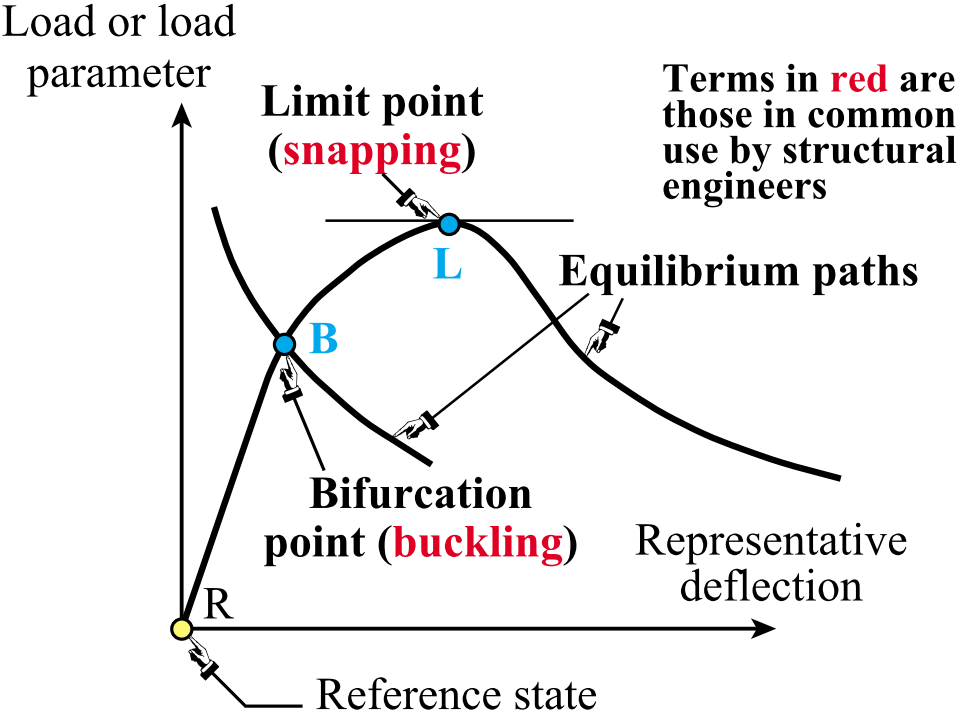
\includegraphics[width=12cm]{images/stability_eq_path.png}
	\caption{Equilibrium paths denoting critical points \cite{FelippaStabilityBasics2016}}
	\label{stab1}
\end{figure}

Instability, whether via buckling or snap-through in nature, only occur at critical points $(\mathbf{u}_c,\lambda_c)$ where the determinant of the stiffness matrix vanishes:

\begin{equation} 
det\big[\mathbf{K}(\mathbf{u}_c,\lambda_c)\big] = 0
\label{eqstab1}
\end{equation}

If the stiffness matrix is decomposed into the material stiffness matrix $\mathbf{K}_m$ (itself composed of the elastic stiffness $\mathbf{K}_e$ and initial displacement stiffness $\mathbf{K}_u$) and the geometric stiffness matrix $\mathbf{K}_g$, the equation above can be expanded:

\begin{equation} 
det\big[
\mathbf{K}_e +
\mathbf{K}_u(\mathbf{u}_0) +
\mathbf{K}_g(\mathbf{u}_c,\lambda_c)
\big] = 
det\big[
\mathbf{K}_m +
\mathbf{K}_g(\mathbf{u}_c,\lambda_c)
\big] = 0
\label{eqstab2}
\end{equation}

It's apparent the expression can be characterized as an eigenvalue problem, thus the eigenvector $\mathbf{z} \neq \mathbf{0}$ corresponding to bifurcation mode shapes can be introduced:

\begin{equation} 
det\big[
\mathbf{K}_m +
\mathbf{K}_g(\mathbf{u}_c,\lambda_c)
\big]\mathbf{z} = 0
\label{eqstab3}
\end{equation}

- Definition

- Examples of where it's important. P-delta effect

- Critical points, det = 0

- Example, just show summary, put full calc in appendix

- Linear prebuckling definiton

- Linear pre-buckling example

- Implementation of LPB